\documentclass{article}
\usepackage[utf8]{inputenc}

\usepackage{graphicx}
\graphicspath{{images/}}

\usepackage{caption}
\usepackage{subcaption}
\captionsetup{compatibility=false}

\usepackage{hyperref}
\hypersetup{
    colorlinks,
    citecolor=black,
    filecolor=black,
    linkcolor=black,
    urlcolor=blue
}

\title{Polytope}
\author{URL, }
\date{February 2021}

\begin{document}

\maketitle

\section{Introduction}
Welcome to the \href{https://discord.gg/invite/zMRu7T4}{Polytope Discord}! Here we discuss \textbf{polytopes}, which is a general term that encompasses polygons (2D), polyhedra (3D), polychora (4D), and so on for any dimension.

\section{Regular polytopes}
There are multiple definitions for when a polytope is \textbf{regular}, but they all require every element (vertices, edges, faces, etc.) to ``look the same.''

\section{Uniform polytopes}
Intuitively, a polytope is \textbf{uniform} when all of its facets are regular and all of its vertices ``look the same.'' To see what we mean, let's look at a few examples.

\begin{figure}[h]
\centering
\begin{subfigure}{.33333\textwidth}
  \centering
  \includegraphics[width=.5\linewidth]{tut}
  \caption{Truncated tetrahedron}
  \label{fig:tut}
\end{subfigure}%
\begin{subfigure}{.33333\textwidth}
  \centering
  \includegraphics[width=.5\linewidth]{did}
  \caption{Dodecadodecahedron}
  \label{fig:did}
\end{subfigure}%
\begin{subfigure}{.33333\textwidth}
  \centering
  \includegraphics[width=.5\linewidth]{snid}
  \caption{Snub icosidodecahedron}
  \label{fig:snid}
\end{subfigure}%
\caption{Three examples of uniform polytopes.}
\label{fig:uniforms3D}
\end{figure}

\section{CRF polytopes}
A polytope is called \textbf{convex regular-faced}, or \textbf{CRF} for short, when it is convex (without dents, holes or self-intersections) and all of its faces are regular. Let's look at a few examples.

\begin{figure}[h]
\centering
\begin{subfigure}{.33333\textwidth}
  \centering
  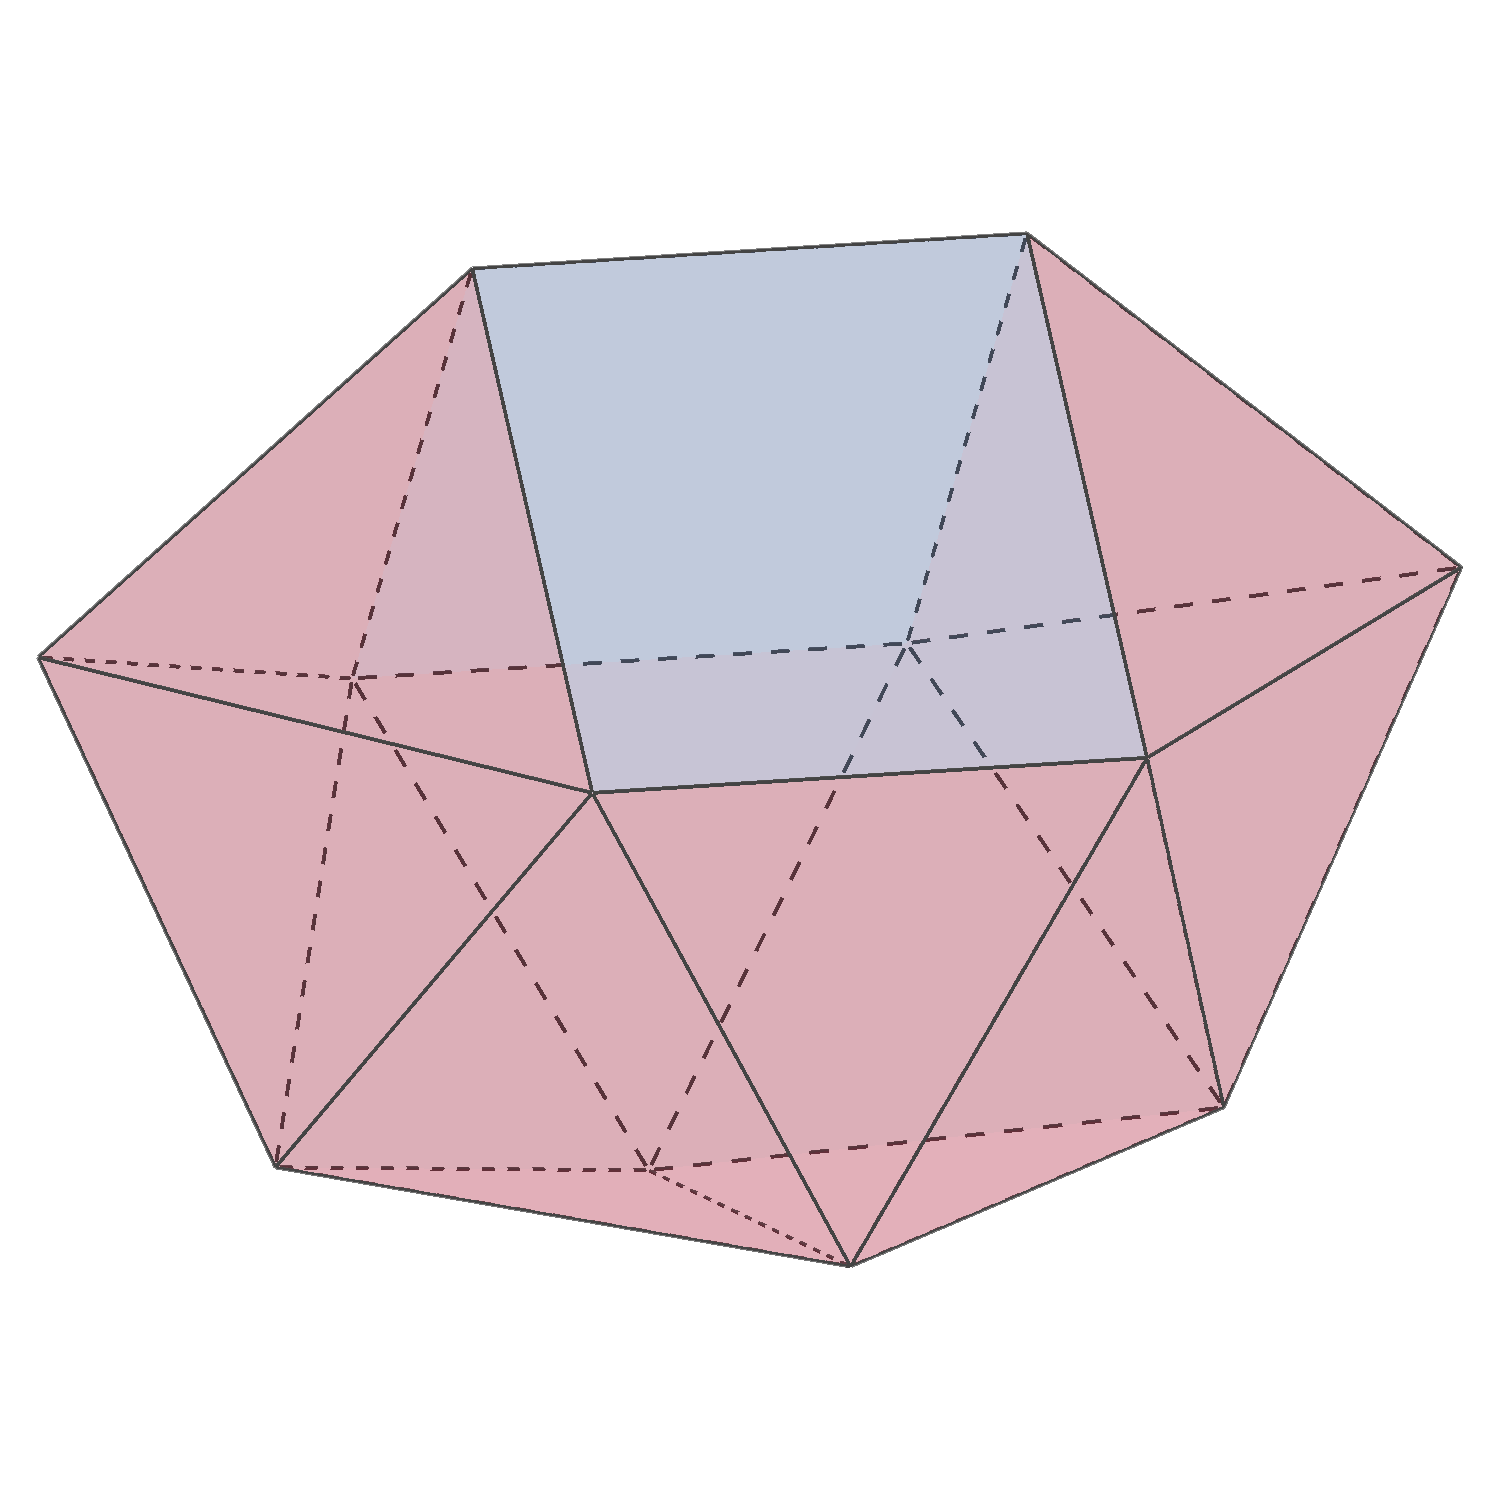
\includegraphics[width=.5\linewidth]{Sphenomegacorona}
  \caption{Sphenomegacorona}
  \label{fig:polyhedra_1}
\end{subfigure}%
\begin{subfigure}{.33333\textwidth}
  \centering
  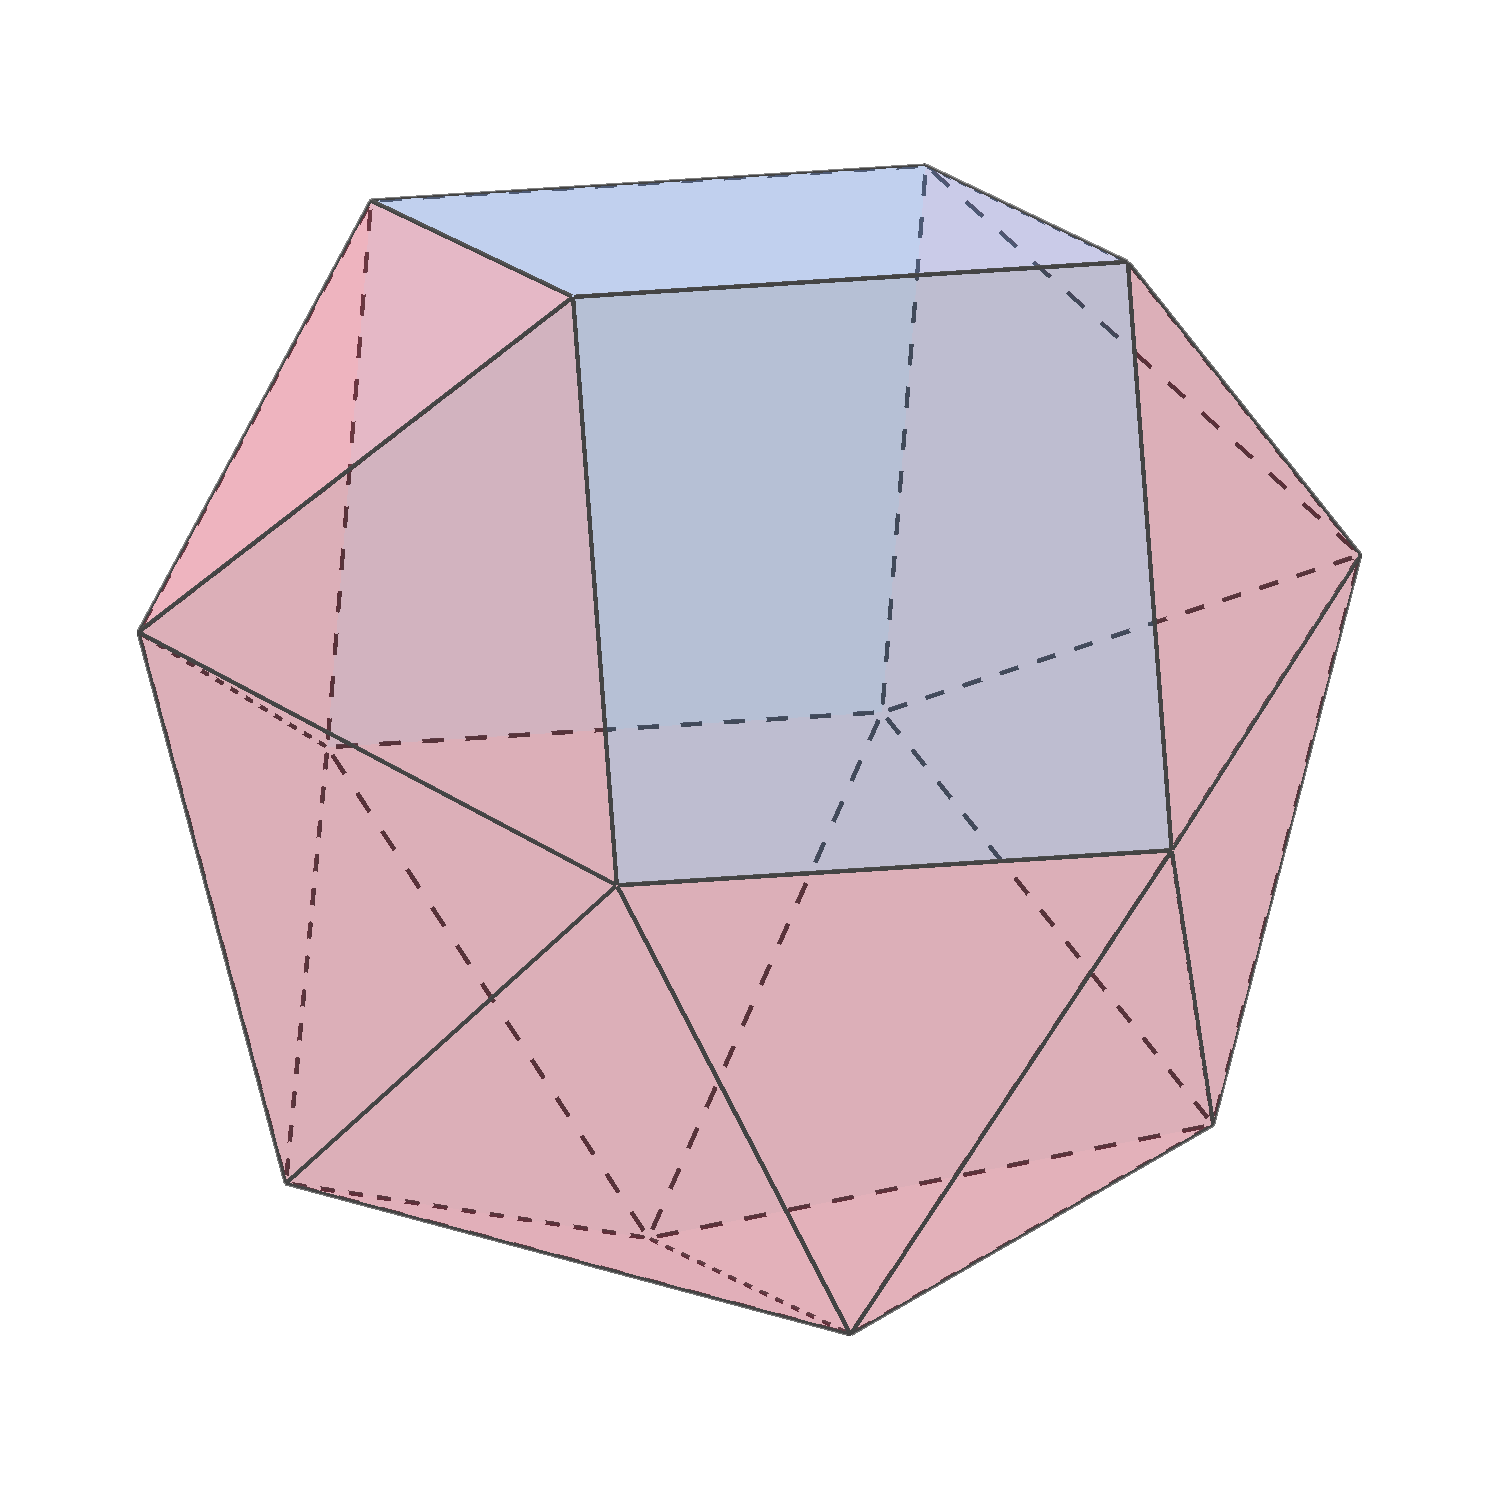
\includegraphics[width=.5\linewidth]{Hebesphenomegacorona}
  \caption{Hebesphenomegacorona}
  \label{fig:polyhedra_2}
\end{subfigure}%
\begin{subfigure}{.33333\textwidth}
  \centering
  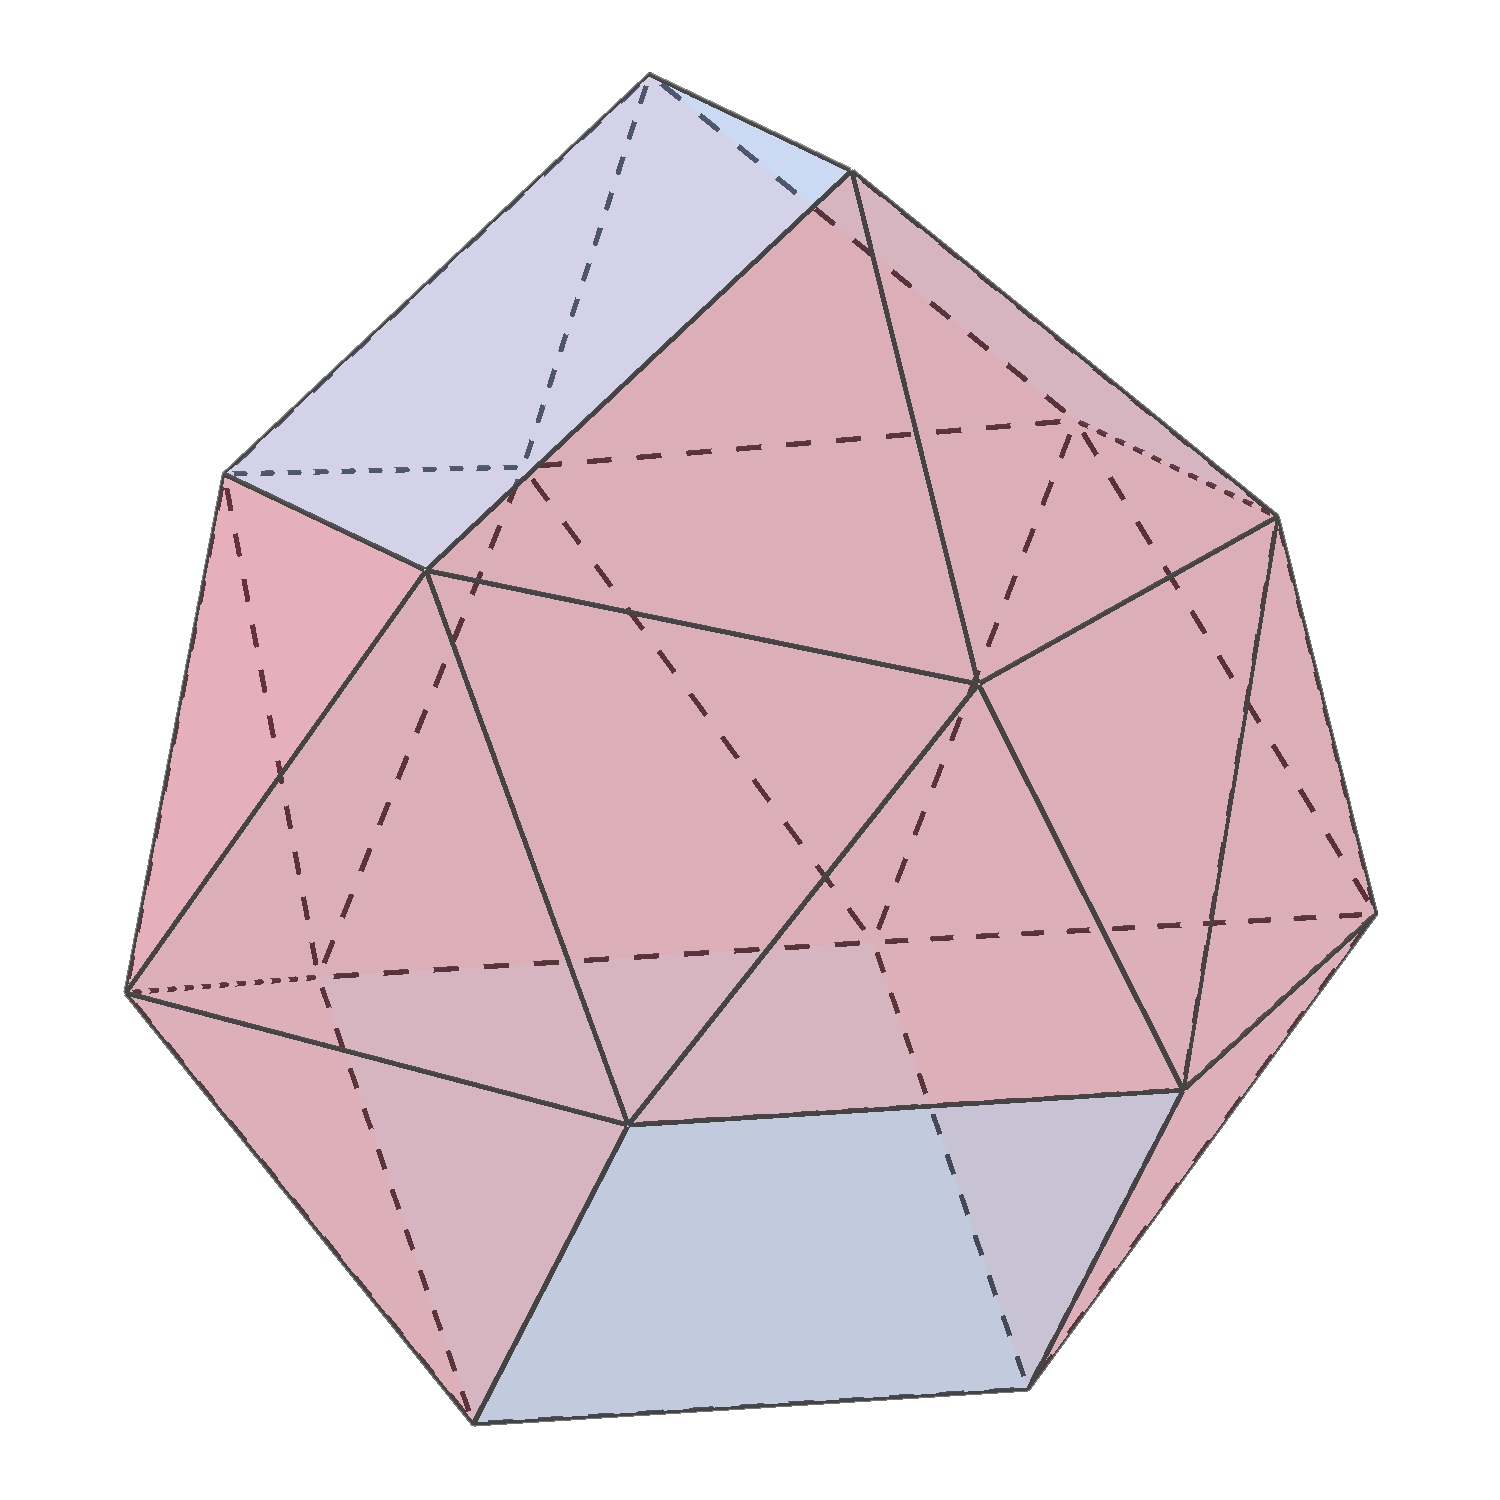
\includegraphics[width=.5\linewidth]{Disphenocingulum}
  \caption{Disphenocingulum}
  \label{fig:polyhedra_3}
\end{subfigure}%
\caption{Test images!}
\label{fig:polyhedra}
\end{figure}


\end{document}
